\chapter{SLOG: A Structural Generalization Test for Semantic Parsing} \label{chp:slog}


\startcontents[chapters]
\printmyminitoc{
}


\noindent In the previous part of this dissertation, we assessed the syntactic capabilities of an autoregressive Transformer, specifically focusing on its ability to handle two syntax-sensitive phenomena. Our findings indicate that the model acquires remarkably nuanced representations of sentence structure, as evidenced by its strong performance on both behavioral-level tasks and measures of representational adequacy when evaluated on unseen, held-out evaluation sets.  


However, this leads us to another critical dimension of inquiry: the nature and depth of the model's observed syntactic generalization. Early studies by \cite{fodor2002compositionality} and \cite{marcus2003algebraic}
posited that neural language models like RNNs may lack the capacity for genuine compositional syntactic generalization due to the absence of explicit symbolic representation. These models, they argued, often rely on similarity-based inference derived from patterns encountered during training. This notion is supported by recent studies, such as \cite{bender2021dangers}, which describe language models as ‘‘stochastic parrots’’ that primarily memorize and shallowly recombine observed examples. Additionally, the capacity for extensive memorization in neural models is well recognized in the literature~\citep{halevy2009unreasonable,zhang2021understanding}.

Let's consider the case of subject-verb agreement across relative clauses, as detailed in Section \ref{sec:two_agreements}. Our findings from Chapter~\ref{chp:main_project} suggest that the Transformer leverages the structural relationships between words to accurately predict the long-distance dependency illustrated in (\ref{ex:slog_s-v}).
\vspace{-0.25\baselineskip}
\begin{exe}
    \ex \label{ex:slog_s-v} \textsc{Target sentence:} \textcolor{orange}{\textbf{NP$_1$}} + \textcolor{blue}{Relative Clause$_1$} + \textcolor{orange}{\textbf{V$_1$}}
    \ex Compositional generalization:
    \begin{xlist}
        \ex \label{ex:S-V_local} \textcolor{orange}{\textbf{NP$_2$}} + \textcolor{orange}{\textbf{V}$_2$}
        \ex \label{ex:N-RC} ... V + \textbf{NP}$_3$ + \textcolor{blue}{Relative Clause$_3$}.
    \end{xlist}
    \ex \label{ex:slog_simi_s-v}Similarity-based generalization:  \textcolor{orange}{\textbf{NP$_4$}} + \textcolor{blue}{Relative Clause$_4$} + \textcolor{orange}{\textbf{V$_4$}}
\end{exe}
\vspace{-0.25\baselineskip}
As proposed by Fodor and Marcus, we can hypothesize two potential ways the model learns such a structural relationship. First, the model might rely on training sentences such as (\ref{ex:S-V_local}) and (\ref{ex:N-RC}). By compositionally combining these structures, the model could infer the long-distance dependency relationship in (\ref{ex:slog_s-v}). This approach exemplifies compositional generalization. Second, the model might extrapolate grammatical knowledge from training sentences like in (\ref{ex:slog_simi_s-v}) to the target sentence (\ref{ex:slog_s-v}) based on their structural similarity. In this process, the model could grasp concepts like syntactic subjecthood, morpho-syntactic number, and the boundaries of relative clauses, subsequently formulating distributional rules at these abstract category levels. By recapitulating its training data through structural similarity and lexico-categorical abstraction, the model can generalize to unfamiliar sentences with known structures. Given that in Chapter~\ref{chp:main_project} we do not control the types of syntactic structures in the model's pretraining data, it is plausible that the model's performance on unseen sentences is driven more by memorization of structures encountered in the training data than by genuine compositional generalization.


This brings us to the core questions: To what extent do these models rely on memorizing structures they have encountered during training? More importantly, can these models achieve generalizable abstractions by compositionally applying observed syntactic rules to interpret new, unseen linguistic patterns? While systematic compositional generalization is a key component in human linguistic cognition, it remains an open question whether these neural models can also dynamically recombine known elements in a compositionally consistent manner with their underlying syntactic structure.



To explore these questions, the current chapter introduces a compositional generalization challenge test. This test aims to directly probe the model's capability to compositionally interpret unseen syntactic constructions through the combination of known structures, and will include experiments with similar Transformer-based models.

\paragraph{Outline} In this chapter,\footnote{This chapter stems from my visiting project at New York University, mentored by Prof. Tal Linzen and Dr. Najoung Kim, and conducted in collaboration with Alexander Koller, Yuekun Yao, and Lucia Donatelli. This chapter draws largely from our paper titled ``SLOG: A Structural Generalization Benchmark for Semantic Parsing'', which I primarily authored and has been accepted by EMNLP 2023.} Section \ref{sec:slog_intro} outlines the foundational aspects of compositional generalization and the semantic parsing task, followed by an introduction to the COGS benchmark \citep{kim-linzen-2020-cogs}, which serves as the starting point of this study. Section \ref{sec:slog_dataset} provides an overview of our SLOG benchmark, a dataset specifically constructed to focus on compositional structural generalization. Section \ref{sec:data_generation} details the dataset generation, and Section \ref{sec:slog_ex_setup} describes the experimental setting, discussing the models evaluated and the evaluation metric. Moving on to Section \ref{sec:slog_res}, we present the findings of our investigation into three Transformers-based models and a structure-informed parsing model. And Section \ref{sec:slog_conclu} provides a summarizing conclusion. 

\section{Introduction} \label{sec:slog_intro}

The immense productivity of human language enables us to understand and produce a potentially infinite number of sentences from finite input elements \citep{chomsky1965aspects, hauser2002faculty}. This linguistic productivity is generally attributed to the principle of compositionality --- the assumption that the meaning of an expression is a function of the meanings of its components and the way they are syntactically combined \citep{frege_1892,partee1984compositionality}. Reflecting this principle, human linguistic competence exhibits \emph{compositional generalization}: the algebraic capacity to understand and produce novel sentences by reassembling known elements \citep{montague1974c}. 

Central to this compositional generalization are two key concepts: \textit{systematicity} and \textit{productivity}, as presented by~\cite{fodor1988connectionism}. Systematicity refers to the consistent application of compositional rules to linguistic elements to derive meaning. This is analogous to how algebraic functions are consistently applied to appropriate variables. In practical terms, systematicity allows humans to extend their understanding to sentences or concepts that are systematically related. Productivity, on the other hand, is the ability to generate an infinite variety of sentences or thoughts from a finite set of words or concepts. In language, this is seen in our ability to produce and understand new sentences that we have never encountered before. 

A classic illustration of this, presented by Fodor, is that people who know the meaning of \emph{John loves Mary}, along with its underlying syntactic rules, can naturally understand the meaning of \emph{Mary loves John}, despite never having encountered it before \citep{fodor1988connectionism}. This exemplifies the systematicity in human language, where understanding such sentences involves the application of the same rules to recombine the same lexical units. In these two sentences, the verb \textit{loves} operates as a function, taking two variables (the subject and the object) and recombining the lexical units \textit{John} and \textit{Mary} in a way that generates different semantic meanings. This rule-based systematic generalization mechanism is widely assumed as the means humans use to handle linguistic productivity. 


Recent advances in NLP, particularly those based on neural networks, do not explicitly rely on the principle of compositionality. Despite this, their empirical success in various tasks suggests that they must have some form of effective generalization. This raises the question: Do these models learn to generalize in a manner similar to human-like compositional understanding, capturing both systematicity and productivity?
In recent years, a growing body of research has explored whether models possess such capability. Benchmarks for compositional generalization in semantic parsing have emerged as a useful tool to assess model's compositional capability \citep{lake2018generalization,hupkes2020compositionality,keysersmeasuring,kim-linzen-2020-cogs}. Semantic parsing tasks in these studies involve translating natural language expressions into semantic representations. The models are evaluated on a \emph{generalization set}, which is sampled from a distribution that systematically differs from the training distribution. This shift from training to evaluation is designed under the principle of compositionality and often includes new combinations of lexical units and observed rules, deeper recursions of observed patterns, or longer sequences. 

\begin{figure}[H]
\vspace{-3mm}  % reduce space above the figure
\captionsetup[subfigure]{font=normalsize}
%\captionsetup{width=0.98\textwidth}
    \centering
    \scalebox{0.78}{
    \begin{subfigure}{0.9\textwidth}
        \centering
    \begin{forest}
        for tree={s sep=5mm,, inner sep=0, l=0,} 
        [,phantom,s sep=2.5cm
        [  S 
            [ NP [Emma]]
            [ VP
                [ V [saw ] ]
                [ NP ,alias=o, tikz={\node [draw, dashed, white,fill=orange!30, fill opacity=0.20, fit=()(!1)(!l)]{}; }
                     [the dog, roof]   
                ]
            ]
        ]
        [S , tikz={\node [draw, dashed,white,fill=blue!30, fill opacity=0.15, fit=()(!11)(!lll)]{};} 
            [NP, alias=w, 
                 [The cat, roof]      
            ]
            [VP, [V,alias=a,[ran, [,no edge] ]
                 ]    
            ]
        ]
        [S , tikz={\node [draw, dashed,white,fill=blue!20, fill opacity=0.15, fit=()(!11)(!lll)]{};} 
            [NP,  tikz={\node [draw, dashed,white,fill=orange!30, fill opacity=0.25, fit=()(!1)(!l)]{};}
                 [The dog, roof]      
            ]
            [VP,
                [V, alias=b, [ran, [,no edge] ]
                ]  
            ]
        ]
        ]
        \tikz[overlay] \node[] (plus) at ($(o)!.5!(w)$) {\scalebox{1.5}{+}};
        \tikz[overlay] \node[] at ($(w)!.5!(b)$) {\scalebox{1.5}{$\leadsto$}};
    \end{forest}
    \caption{Lexical generalization: object $\rightarrow$ subject (COGS) } \label{fig:cogs_lex_gen}
    \end{subfigure}}
    \scalebox{0.75}{
    \begin{subfigure}{0.9\textwidth}
        \centering
        \begin{forest}
        for tree={s sep=2mm,, inner sep=0, l=0}
        [,phantom,s sep=3cm
        [S 
            [NP [Emma]]
            [VP
                [V [saw ]]
                [NP, tikz={\node [fill=green!30, fill opacity=0.25, fit=()(!1)(!l)]{};} 
                    [NP,  [the dog, roof]]
                    [PP, 
                        [P [on]]
                        [NP, alias=a,tikz={\node [fill=green!30, fill opacity=0.25, fit=()(!1)(!l)]{};}
                            [NP,  [a mat, roof]]
                            [PP,  [in a box, roof]]
                        ]
                    ]
                ]
            ]
        ]
        [S 
            [NP [Emma]]
            [VP
                [V [saw ]]
                [NP, tikz={\node [fill=green!30, fill opacity=0.25, fit=()(!1)(!l)]{};} 
                    [NP, alias=b, [the dog, roof]]
                    [PP
                        [P, [on]]
                        [NP, tikz={\node [fill=green!30, fill opacity=0.25, fit=()(!1)(!l)]{};}
                            [NP,  [a mat, roof]]
                            [PP 
                                [P [in]]
                                [NP,tikz={\node [fill=green!30, fill opacity=0.25, fit=()(!1)(!l)]{};}
                                    [NP, [a box, roof]]
                                    [PP, [in a house, roof]]
                                ]
                            ]
                        ]
                    ]
                ]
            ]
        ]
        ]
    \tikz[overlay] \node[] at ($(a)!.5!(b)$) {\scalebox{1.5}{$\leadsto$}};
    \end{forest}
    \captionsetup{skip=2em} 
    \caption{Structural generalization: deeper recursion depths (COGS \& SLOG) } \label{fig:cogs_struc_gen}
    \end{subfigure}}
        \scalebox{0.75}{
    \begin{subfigure}{0.9\textwidth}
        \centering
    \begin{forest}
        for tree={s sep=3mm,, inner sep=1, l=0}
        [, phantom, s sep=2.5cm
        [,phantom,s sep=3.5cm
        [S 
            [NP [Emma]]
            [VP 
                [V [saw ] ]
                [NP , alias=o, tikz={\node [draw, dashed, white,fill=green!30, fill opacity=0.20, fit=()(!1)(!ll)]{};}
                    [NP  [the dog, roof]]
                    [RC ,alias=e, [that Max held \_, roof]   
                    ]
                ]
            ]
        ]
        [S , tikz={\node [draw, dashed,white,fill=blue!30, fill opacity=0.15, fit=()(!11)(!lll)]{};} ,alias=h,
            [NP , alias=w,
                 [The cat, roof]  
            ]
            [VP
                [V, [ran, [,no edge] ]
                ] 
            ]
        ]
        ]
        [, phantom, s sep=2.5cm
        [S, tikz={\node [draw, dashed,white,fill=blue!30, fill opacity=0.15, fit=()(!111)(!lll)]{};}
            [NP , tikz={\node [fill=green!30, fill opacity=0.25, fit=()(!11)(!ll)]{};}
                [NP, [The dog, roof]]
                [ RC,alias=b,   [that Max saw \_, roof]
                ]
            ]
            [VP
                 [V, [ran, [,no edge] ]
                ] 
            ]
        ]
        ]
        ]
        \tikz[overlay] \node[] (plus) at ($(o)!.6!(w)$) {\scalebox{1.5}{+}};
        \tikz[overlay] \node[] at ($(w)!.4!(b)$) {\scalebox{1.5}{$\leadsto$}};
    \end{forest} 
    \caption{Structural generalization: RC object $\rightarrow$ RC subject (SLOG) }  \label{fig:slog_struc_gen}
    \end{subfigure}}
    \caption{
    Examples of lexical generalization in COGS --- (a), and structural generalization in COGS --- (b) and in SLOG --- (b, c). The SLOG task requires mapping the generalization examples to their logical forms; the corresponding logical forms are shown in Table~\ref{tab:cogs-lf}. 
    }
    \label{fig:lex_struc_gen}
    \vspace{-3mm}
\end{figure}

The COGS (\textbf{CO}mpositional \textbf{G}eneralization
Challenge based on \textbf{S}emantic Interpretation) dataset \citep{kim-linzen-2020-cogs} in particular has become a widely used benchmark, as it is designed to expose a generalization gap between training and testing data that many recent semantic parsers still struggle with. COGS distinguishes two types of generalization challenges that require different types of algebraic compositional strategies: \textit{lexical generalization} tests the ability to interpret novel combinations of known lexical items and known linguistic structures (Figure~\ref{fig:cogs_lex_gen}), and \textit{structural generalization} tests the ability to combine known structures into a novel structure (Figure~\ref{fig:cogs_struc_gen} and~\ref{fig:slog_struc_gen}). Importantly, the majority of generalization types in COGS target lexical generalization (18 of 21 generalization types, 86\% of the dataset). As lexical generalization is arguably easier than structural generalization (e.g., solvable by simple slot-filling), this imbalance may lead to overall performance numbers that are overly optimistic with regard to a model's capacity to generalize compositionally, as pointed out by \cite{weissenhorn-etal-2022-compositional} and \cite{yao-koller-2022-structural}. 




To facilitate a more comprehensive evaluation of structural generalization, we introduce SLOG, a \textbf{S}tructural \textbf{LO}ng-distance dependencies \textbf{G}eneralization benchmark. SLOG extends COGS to include 17 cases of structural generalization in total (14 new cases and 3 existing cases from COGS) (\S\ref{sec:slog_dataset}). The novel generalizations we introduce target two key structural features of human language: recursion and filler-gap dependencies.

Prior research has extensively investigated the processing of recursive constructions, a key feature of human language enabling the creation of complex, nested structures and hierarchical relationships~\citep{hauser2002faculty}. This area of study spans both artificial neural networks and human cognition \citeti{christiansen1999toward,lakretz2021can,mccoy2021infinite}.
Using artificial languages to isolate syntactic properties, research has shown that humans can learn and extrapolate nested patterns to deeper levels \citep{mccoy2021infinite}. In contrast, the capabilities of Transformer-based models in capturing recursive regularities have yielded mixed results \citep{bhattamishra-etal-2020-ability,hahn:2020,ebrahimi-etal-2020-self,lakretz2021can}. For filler-gap dependencies, a particularly challenging type of long-distance dependency involves generalization about the absence of material. Prior work has centered on syntactic tasks involving \textit{wh}-questions or relative clauses \citeti{wilcox-etal-2018-rnn,marvin-linzen-2018-targeted,li-etal-2023-assessing}. These studies primarily use language modeling as the task and do not 
require mapping to semantic representations. SLOG diverges from these works by incorporating recursion and filler-gap dependency in a more naturalistic setting and directly assess the semantic mapping. Importantly, rather than isolating syntactic generalization from linguistic meaning, our approach aims to assess whether models rely on syntactic generalization that aligns with human inductive biases to derive the meaning of complex sentences.

We use SLOG to evaluate a Seq2Seq Transformer model trained from scratch \citep{NIPS2017_3f5ee243}, two pre-trained Transformers (T5-base; \citealt{2020t5} and LLaMA; \citealt{touvron2023llama}), and a structure-informed\footnote{In this study, `structure-informed' refers specifically to models that incorporate explicit representations of linguistic structure.} model (AM-Parser; \citealt{weissenhorn-etal-2022-compositional}). In comparison to their overall performance on COGS, all models exhibit considerably lower performance on SLOG (\S\ref{sec:slog_res}). The generalization accuracy of Transformer-based models, including pre-trained ones, only reaches 40.6\%, and even a structure-informed parser, while exhibiting near-perfect generalization on COGS structural cases, only achieves 70.8\% on SLOG. The cases in which models struggle exhibit distinct patterns and suggest varied approaches of models to solving the task. An error analysis reveals that the AM-Parser generalizes well on existing structural generalization cases in COGS but struggles with the gap constructions introduced in SLOG due to inherent structural limitations, which we discuss in Section~\S\ref{subsec:am_parser_analysis}. Transformers tend to erroneously repeat frequent meaning representation subsequences observed during training. Even with pretraining, they struggle with unseen long-distance dependencies, which we attribute to their bias towards shorter predicate-argument dependencies~(\S\ref{subsec:long_distance_hard}). 

Overall, the discrepancy in performance between SLOG and COGS illuminates the notable gap between models' lexical and structural generalization abilities. It highlights the utility of SLOG in exposing the limitations of current models that have been shown to achieve high performance on existing generalization benchmarks, and helps foreground the different weaknesses of these models. While Transformer-based models can approximate compositional behavior to a certain extent, our findings suggest that they do not seem to rely on the kind of syntactic generalization rooted in symbolic compositional rules, which are believed to drive human linguistic systematicity and productivity. 


\section{Overview of SLOG benchmark} \label{sec:slog_dataset}
SLOG follows the semantic parsing format used in COGS, where the task is to translate English expressions into logic-based meaning representations (Table~\ref{tab:cogs-lf}). The dataset structure follows the basic design principles of COGS: there is a systematic gap between the training set and the generalization set, where target constructions in the generalization set are not included in the training set, but pieces of the training set can be recombined to arrive at their correct meanings. For example, as illustrated in example (c) of Table~\ref{tab:cogs-lf}, noun phrases that appear only in object position during training must be reinterpreted in subject position during generalization. 







\begin{table*}[htb!]
    \small
    \centering
    \setlength{\tabcolsep}{3pt}
    \begin{tabularx}{\linewidth}{p{12mm}>{\raggedright\arraybackslash}X @{\hspace{0.7em}} >{\raggedright\arraybackslash}X}
    \toprule
        & \textbf{Training}  
        & \textbf{Generalization} \\ 
        \midrule
        COGS
         & (a)The cat \textbf{ran}. \newline $\leadsto$ \lform{*cat($x_1$); run.agent($x_2,x_1$)} \newline
         Emma saw \textbf{the dog}.  \newline
         $\leadsto$ \lform{*dog($x_3$);see.agent($x_1,$Emma) $\land$ see.theme($x_1, x_3$)} 
         &  \textbf{The dog} ran. \newline
        $\leadsto$ \lform{*dog($x_1$); run.agent($x_2,x_1$)} \\ 
         %\cmidrule(l){2-3}
         \midrule
        \makecell[tc]{COGS \\ \&\\ SLOG} & (b) Emma saw the dog \textbf{on a mat in a box}.  \newline
        $\leadsto$ \lform{*dog($x_3$);see.agent($x_1,$Emma) $\land$ see.theme($x_1, x_3$) dog.nmod.on($x_3,x_6$) $\land$ mat($x_6$) $\land$ mat.nmod.in($x_6,x_9$) $\land$ box($x_9$)} 
         &  Emma saw the dog \textbf{on a mat in a box in a house}. \newline
         $\leadsto$\lform{*dog($x_3$);see.agent($x_1,$Emma) $\land$ see.theme($x_1, x_3$) dog.nmod.on($x_3,x_6$) $\land$ mat($x_6$) $\land$ mat.nmod.in($x_6,x_9$) $\land$ box($x_9$) $\land$ box.nmod.in($x_9,x_{12}$) $\land$ house($x_{12}$)} \\ 
        \midrule
         SLOG 
         &(c) The cat \textbf{ran}. \newline $\leadsto$ \lform{*cat($x_1$); run.agent($x_2,x_1$)}\newline
         Emma saw \textbf{the dog that Max held}. \newline 
         $\leadsto$ \lform{*dog($x_3$); see.agent($x_1,$Emma) $\land$ see.theme($x_1, x_3$) $\land$ dog.nmod($x_3,x_6$) $\land$ hold.agent($x_6,$Max) $\land$ hold.theme($x_6,x_3$)} 
         
         &  \textbf{The dog that Max saw} ran. \newline
         $\leadsto$ \lform{*dog($x_1$); see.agent($x_4,$Max) $\land$ see.theme($x_4,x_1$) $\land$ dog.nmod($x_1,x_4$) $\land$ run.agent($x_5,x_1$)} \\ 
         \bottomrule
    \end{tabularx}
    \caption{
        Examples of two distinct types of generalization: lexical generalization in COGS --- (a), structural generalization in COGS---(b) and in SLOG --- (b, c). The symbol $\leadsto$ indicates the task of translating an English sentence into its corresponding meaning representation.
    }\label{tab:cogs-lf}
\end{table*}



SLOG is generated using manually specified rules (\S\ref{sec:data_generation}), adopting the same meaning representation as COGS. The COGS \ac{LF}, derived from \cite{reddy-etal-2017-universal}, is based on Neo-Davidsonian view of verbal arguments. In this approach, the semantic units are mapped to indexed variables. For example, in: 
\vspace{-0.5\baselineskip}
\begin{exe}
    \ex The cat \textbf{ran}. \newline $\leadsto$ \lform{*cat($x_1$); run.agent($x_2,x_1$)} 
\end{exe}
\vspace{-0.5\baselineskip}
The variable \texttt{$x_1$} denotes an entity that is both a cat and the agent of a running event, while \texttt{$x_2$} represents the running event. The variable indices are determined by the linear position of the phrasal head in the input sentence. For example, \textit{cat} corresponds to $x_1$, since, under 0-indexing, \textit{cat} appears in linear position 1 of the English sentence \textit{The cat ran}. Definite descriptions are marked by a preceding asterisk and are placed at the beginning of the LF: \lform{*cat($x_1$)} is separated from the remaining conjuncts by a `;'.\footnote{Proper nouns, treated as constants, are not represented by numbered variables but by their actual word forms as illustrated in the example (\ref{ex:corefer_rc}).} This format can represent coreferential relations effectively, for example:
\begin{exe}
    \ex \label{ex:corefer_rc} Emma saw \textbf{the dog that Max held \_\_}. $\leadsto$  \newline 
         \lform{*dog(\textcolor{blue}{$x_3$}); see.agent($x_1$, Emma) $\land$ see.theme($x_1$, \textcolor{blue}{$x_3$}) $\land$ dog.nmod($x_3,\ x_6$) $\land$ hold.agent($x_6$, Max) $\land$ hold.theme($x_6$, \textcolor{blue}{$x_3$})} 
\end{exe}
The variable \texttt{$x_3$} denotes a \textit{dog} entity that is both the theme of a seeing event in the main clause and the theme of a holding event in the relative clause.



SLOG contains 17 structural generalization cases grouped into four categories. These generalization cases are primarily motivated by frequency asymmetries in natural language, where simpler structures are more common than complex ones; in other words, SLOG assesses whether NLP models can extrapolate from frequent patterns to their less frequent counterparts. We describe the four categories below; see Table~\ref{tab:gen_cases} for the full list of generalization cases.



\begin{table}
\centering
%\setlength{\extrarowheight}{-4pt} %reduce space between rows
\captionsetup{width=\textwidth}
\renewcommand{\arraystretch}{1.0} % adjust row spacing
\scalebox{0.76}{
\begin{tabular}{p{0.4\textwidth}p{0.37\textwidth}p{0.4\textwidth}}
\toprule 
Generalization cases & Training & Generalization  \\
\midrule 

\multicolumn{3}{c}{\ \textsection\ref{subsec:cat_recur} Novel Recursion Depth} \\
\midrule

\multicolumn{3}{l}{\textit{Deeper depth generalization}} \\

$\checkmark$\makecell[tl]{\ac{PP} \\ max depth 4 $\rightarrow$ depth 5-12} & Ava saw the ball {\bf in} the bottle {\bf on} the table. & Ava saw the cat {\bf in} the box {\bf on} the mat {\bf on} the bed {\bf on} the floor {\bf in} the room. \\

$\checkmark$\makecell[tl]{Tail CP recursion \\ max depth 4 $\rightarrow$ depth 5-12}  & Ava believed \textbf{that} Emma said \textbf{that} a fish froze.  & Ava said \textbf{that} Emma liked \textbf{that} Max believed \textbf{that} Noah found \textbf{that} Liam saw \textbf{that} the cat slept. \\

 \phantom{$\checkmark$} \makecell[tl]{Center embedding \\
max depth 4 $\rightarrow$ depth 5-12} & Eva saw the cat \textbf{that} the horse \textbf{that} the dog liked chased. & Ava held the dress \textbf{that} a store \textbf{that} a girl \textbf{that} a boy \textbf{that} a cat \textbf{that} a man drew saw loved knew sold.  \\

\multicolumn{3}{l}{\textit{Shallower depth generalization}} \\

\phantom{$\checkmark$} \makecell[tl]{PP recursion \\
max depth 4 $\rightarrow$ depth 3}  & Emma saw the ball {\bf in} the bottle {\bf on} the table {\bf on} the floor {\bf in} the office. & Ava saw the cat {\bf on} the mat {\bf on} the floor {\bf in} the office. \\

\phantom{$\checkmark$} \makecell[tl]{Tail CP recursion \\
max depth 4 $\rightarrow$ depth 3} & Ava believed \textbf{that} Emma said \textbf{that} Max found \textbf{that} a cat saw \textbf{that} a fish froze.  & Ava said \textbf{that} Emma liked \textbf{that} Max believed \textbf{that} the cat slept. \\

\phantom{$\checkmark$} \makecell[tl]{Center embedding \\
max depth 4 $\rightarrow$ depth 3} & Eva saw the cat \textbf{that} the horse \textbf{that} the dog  \textbf{that} the man \textbf{that} the girl loved found liked chased. & Emma bought the dress \textbf{that} the store \textbf{that} the woman \textbf{that} Mike knew liked sold.  \\
\midrule
\multicolumn{3}{c}{ \textsection\ref{subsec:cat_mod} Novel Combination of Modified Phrases and Grammatical Roles} \\ \midrule 
\multicolumn{3}{l}{PP in direct object NPs} \\

 $\checkmark$$\rightarrow$ PP in subject NPs  & Noah ate {\bf the cake on the plate}. & {\bf The cake on the table} burned. \\

  %\makecell[l]{PP in direct object \\ $\rightarrow$ PP in indirect object} 
 \phantom{$\checkmark$}$\rightarrow$ PP in indirect object NPs & Noah ate {\bf the cake on the plate}. & Max gave a fish to {\bf a cat on a table}. \\
  \multicolumn{3}{l}{PC in direct object NPs} \\
 \phantom{$\checkmark$}$\rightarrow$ RC in subject NPs & Noah saw {\bf the cat that froze}. & {\bf The cat that froze} smiled. \\

\phantom{$\checkmark$}$\rightarrow$ RC in indirect object NPs    & Noah saw {\bf the cat that froze}. & Max gave a fish to {\bf a cat that ran}. \\
\midrule 

\multicolumn{3}{c}{\ \textsection\ref{subsec:cat_gap} Novel Gap positions} \\ 
\midrule 

\makecell[lt]{Subject, direct object-extracted RC \\ 
$\rightarrow$ Indirect object-extracted RC}  & Noah saw the cat that gave a fish to Liam. $\oplus$ Noah saw the cat that Liam liked {\bf \_}. & Noah saw the cat that Emma gave a cake to {\bf \_ }. \\

Subject, direct object \textit{wh}-questions $\rightarrow$ Indirect object \textit{wh}-questions &  \makecell[lt]{Who saw the cat? \\ $\oplus$  What did Emma see {\bf \_}?} & Who did Noah give the cake to {\bf \_}? \\
\midrule 

\multicolumn{3}{c}{ \textsection\ref{subsec:cat_Q} Novel \textit{Wh}-questions} \\ 
\midrule

\multicolumn{3}{l}{Subject, object \textit{wh}-Q of simple transitives} \\

$\rightarrow$ Active subject \textit{wh}-questions & \makecell[l]{{\bf Who saw} the cat? \\ $\oplus$ Emma {\bf wanted} to sleep.}   &  {\bf Who wanted} to sleep ? \\

$\rightarrow$ Passive subject \textit{wh}-questions &  \makecell[l]{ {\bf Who} did Emma see \_? \\ $\oplus$  The boy {\bf was found} by Emma.} &   {\bf Who was helped} by Emma? \\

\makecell[l]{$\rightarrow$ Direct object \textit{wh}-questions \\ \phantom{$\checkmark$} with ditransitive verbs} & \makecell[l]{{\bf What } did Emma see \_? \\ $\oplus$ Emma {\bf gave} a fish {\bf to} the cat.} & {\bf What} did Emma {\bf give} \_ to the cat?  \\

$\rightarrow$ \textit{Wh}-questions with modified NPs &  \makecell[l]{ What did {\bf the cat} see \_? \\ $\oplus$ the cat {\bf on the mat} } & What did {\bf the cat on a table} see \_? \\

$\rightarrow$ \textit{Wh}-questions long movement & {\bf What} did the cat {\bf see} \_? $\oplus$  Emma {\bf said that} the cat saw a fish. & {\bf What} did Emma {\bf say that} the cat {\bf found} \_? \\

\bottomrule 
\end{tabular}
}
\caption{A full list of SLOG generalization cases. Each sentence in the table corresponds to a (sentence, logical form) pair, as illustrated in Figure~\ref{tab:cogs-lf}. $\oplus$ denotes the combination of two observed structures, which allows to interpret the target novel structure. Some cases cover multiple sub-case constructions: e.g. all ditransitive verbs include both double-object and prepositional constructions. Due to space limitations, only one example is provided for each case. The three cases marked with `$\checkmark$' are already present in the COGS dataset.
\label{tab:gen_cases}}
\end{table}


\subsection{Novel recursion depth} \label{subsec:cat_recur}
Recursion allows small, hierarchical phrases to be combined to create larger phrases composed of identical substructures. This combination process can be repeated an unbounded number of times. The COGS dataset tests a model's ability to apply recursion via two cases: sentential complements (e.g. (\ref{ex:nested_CP}); tail \ac{CP} recursion henceforth) and nominal prepositional phrase modifiers (e.g. (\ref{ex:nested_PP}); PPs recursion henceforth). For both cases, the training set
contains recursive depths of 0--2 (0 indicating no PP/CP), and the generalization set
contains strictly greater depths of 3--12.
\begin{exe}
    \ex \label{ex:nested_CP} Tail CP recursion depths 2: 
    \vspace{0.1cm} \\
    \ Mary knows [that John knows [that Emma cooks]$_{CP}$ ]$_{CP}$ 
    \ex \label{ex:nested_PP} PP recursion depths 2: 
    \vspace{0.1cm} \\
    Ava saw the ball [in the bottle [on the table]$_{PP}$]$_{PP}$
\end{exe}

By contrast, the SLOG training set includes recursion of depth 0--2 and 4, and the generalization set contains both an intermediate depth of 3 and deeper depths of 5--12. Including both shallower and deeper embeddings allows us to determine if any difficulty in generalizing to an unseen embedding depth is a consequence of the model's more general difficulty in processing longer sequences than observed in training \citep{lake2018generalization,herzig2021unlocking,anil2022exploring} rather than a more specific issue with applying recursion to generate novel constructions.

In addition to this new depth split, SLOG introduces a new recursion construction. 
COGS involves only tail recursion, which features recursive PPs and CPs with right-branch embeddings. SLOG extends this with center embedding, where a phrase is embedded in the middle of another phrase of the same type, leaving elements on both side of the embedded component and producing well-parenthesized long-distance dependencies, as illustrated by the subscripts in (\ref{ex:center_embed}).

\begin{exe}
    \ex \label{ex:center_embed}  Eva saw the mouse [that the cat$_1$ [ that the dog$_2$  chased$_2$ ] held$_1$ ].
\end{exe}
\noindent At the same recursion depths, the average LF length increases from PP recursion to tail CP recursion to center embedding. 

In natural language, the depth of recursion is rarely greater than five and center embedding is generally limited to two levels~\citep{karlsson2007constraints,karlsson2010syntactic}. SLOG tests deeper recursive patterns up to depth 12. While this may surpass human processing abilities for reasons presumed to be linked to memory constraints \citep{gibson1999memory,karlsson2007constraints}, deeper embedding depth remains grammatical, echoing Chomsky’s competence versus performance distinction. Importantly, we also note that our goal with SLOG is to assess the linguistic competence of NLP models and to investigate whether they achieve their performance through human-like inductive biases that favor compositional generalization. Testing at these greater depths allows us to more comprehensively probe the models' capabilities and limitations. 

\subsection{Novel combination of modified phrases and grammatical roles} \label{subsec:cat_mod}

SLOG also tests the capacity to generalize complex NPs to new syntactic positions. SLOG introduces relative clause modifiers, in addition to PP modifiers already included in COGS.
%\vspace{-0.5\baselineskip}
\subsubsection{Prepositional Phrase modifiers} \label{subsubsec:pp-mod}

The most challenging case in COGS involves interpreting prepositional phrases (PPs) within subject NPs~(\ref{ex:subj_pp}), while the training set only contains PPs within direct object NPs~(\ref{ex:dobj_pp}). Recent Seq2Seq models consistently failed to handle this case~\citep{akyurek-andreas-2021-lexicon,zheng-lapata-2022-disentangled,yao-koller-2022-structural}. To further investigate what makes this challenging generalization hard for models, we take a two-fold approach in SLOG. First, we additionally include generalization targeting indirect object modification, as illustrated in (\ref{ex:iobj-pp}).

\begin{exe}
    \ex \label{ex:subj_pp}[The {\bf cat} on the mat]$_{\textcolor{blue}{subj}}$ {\bf ran}. 
    \ex \label{ex:dobj_pp}Emma saw [the cat on a table]$_{\textcolor{blue}{dobj}}$.
    \ex \label{ex:iobj-pp}Sub-cases of indirect object modification:
    \begin{xlist}
        \ex \label{ex:iobj}Emma {\bf gave} [a cat on the mat]$_{\textcolor{blue}{iobj}}$ a {\bf fish}.
        \ex \label{ex:iobj_dat2} Emma gave a fish to [a cat on the \mbox{mat ]$_{\textcolor{blue}{iobj}}$}. 
        \ex \label{ex:iobj_dat3} A fish was given to [a cat on the \mbox{mat ]$_{\textcolor{blue}{iobj}}$}.
    \end{xlist}
\end{exe}

\noindent We expect sub-cases of indirect object modification to pose challenges of varying difficulty, depending on the distance of the predicate-argument dependency. % expressed in the target sentences. 
For example, generalization to indirect object modification in active oblique datives (\ref{ex:iobj}) introduces an unobserved long-distance dependency between the verb \textit{gave} and the direct object \textit{a fish} across a non-argument NP \textit{the mat}.\footnote{This observation holds true for the generalization to subject modification shown in (\ref{ex:subj_pp}).} In contrast, sub-cases like (\ref{ex:iobj_dat2}) and (\ref{ex:iobj_dat3}), where the non-argument NP \textit{the mat} occurs at the end of the sentences, do not introduce this kind of predicate-argument dependency across an intervening NP and are therefore expected to be relatively easier. 
  

Second, SLOG's training set additionally includes standalone PP-modified NPs, as exemplified in~(\ref{ex:standalone_PP}), to prevent modifiers from being associated with only a particular range of token indices, as pointed out by \citet{wu2023recogs}: In COGS, PPs were restricted to the object position, such as in (\ref{ex:train_PP_dobj}), where the modifier conjunct in the logic form --- \texttt{cat.nmod.on ($x_{i}, x_j$)} --- applies only for i>=3, so models never observed the association of modifiers with linearly-earlier indices (e.g., in (\ref{ex:PP_subj}), \texttt{cat.nmod.on ($x_{i}, x_j$)}, with i=1 ). This makes it difficult to isolate the impact of indices correlation from structural generalization. The inclusion of such fragments in SLOG, absent in COGS but common in child-directed speech~\citep{wells1981learning,cameron2003construction}, serve as a signal that the range of variables indices associated with PP modifiers is not restricted to the object position.\footnote{This phenomenon is also evident in the \href{https://childes.talkbank.org/}{CHILDES} corpora, where we observed many standalone PP-modified NPs (e.g., \textit{the CD on the desk!}) in child-directed speech.}

\begin{exe}
    \ex \label{ex:train_PP_COGS} \textsc{COGS Training} 
    \begin{xlist}
    \ex \label{ex:train_PP_dobj} Emma saw the cat on a table $\leadsto$ \lform{*cat($x_3$); see.agent($x_1,$ Emma) $\land$ \\ see.theme($x_1,x_3$) $\land$ cat.nmod.on($\textcolor{blue}{\bf x_3},x_6$) $\land$ table($x_6$)}
    \ex The dog ran. $\leadsto$ \lform{*dog($x_1$); run.agent($x_2,x_1$)}
    \end{xlist}
\ex \label{ex:train_PP_SLOG}\textsc{SLOG Training} 
\begin{xlist}
  \ex \label{ex:standalone_PP} the cat on a table $\leadsto$ \lform{*cat($x_1$); cat.nmod.on($\textcolor{orange}{\bf x_1},x_4$) $\land$ table($x_4$)}
  \ex \textsc{COGS Training} 
\end{xlist} 
\ex \label{ex:PP_subj} \textsc{Generalization}
 \\
 The cat on a mat ran. $\leadsto$ \lform{*cat($x_1$); cat.nmod.on($\textcolor{orange}{\bf x_1},x_4$) $\land$ map($x_4$)} $\land$ run.agent ($x_5,x_1$)

\end{exe}

\subsubsection{Relative clause modifiers} \label{subsubsec:rc-mod}

Similar to PP modifiers, NPs with relative clause (RC) modifiers, as in (\ref{ex:RC_filler_gap}), can occupy any position that an unmodified NP can fill. We expect RC modifiers to pose a greater challenge compared to PP modifiers, as they involve \textit{gap constructions}, in which a phrase needs to be interpreted in a position other than its canonical position in a declarative clause --- we will refer to this as \textit{extraction} \citep{sag2010english}. We mark gap positions with an underscore. In (\ref{ex:RC_filler_gap}), \textit{the dog} should be interpreted as if it occupies the gap position as the direct object of \textit{held}; in the logical form, this is represented by the fact that $x_3$ is filling both \lform{see.theme} and \lform{hold.theme}.
\vspace{-0.5\baselineskip}
\begin{exe}
     \ex \label{ex:RC_filler_gap} Emma saw the dog that Max held \_\_.  \vspace{0.1cm} \\
         $\leadsto$
         \lform{*dog(\textcolor{blue}{$x_3$}); see.agent($x_1$, Emma) $\land$ \textbf{see.theme}($x_1,$ \textcolor{blue}{$x_3$}) $\land$ dog.nmod($x_3, x_6$) $\land$ hold.agent($x_6,$ Max) $\land$ \textbf{hold.theme}($x_6,$ \textcolor{blue}{$x_3$})} 
    %\ex \label{ex:standalone_RC} the cat that Liam fed \_\_
\end{exe}



\noindent To test for generalization to RC-modified NPs in unseen grammatical roles, SLOG's training set contains RC modifiers in direct object NPs (\ref{ex:RC_obj}) as well as standalone RC-modified NPs like (\ref{ex:standalone_RC}), and the generalization set contains RC modifiers in subject NPs such as (\ref{ex:RC_subj}) and indirect object NPs (\ref{ex:RC_iobj}). This is analogous to the PP modifier cases.
\vspace{-0.5\baselineskip}
\begin{exe}
\ex \label{ex:train_RC}\textsc{Training} 
\begin{xlist}
  \ex \label{ex:standalone_RC} the cat that Liam fed \_\_
  \ex \label{ex:RC_obj} Emma saw [the cat that Max held \_\_]$_{\textcolor{blue}{dobj}}$
\end{xlist} 
\ex \textsc{Generalization}
\begin{xlist}
    \ex \label{ex:RC_subj} [The cat that Emma found \_\_]$_{\textcolor{blue}{subj}}$ smiled.
    \ex \label{ex:RC_iobj} Liam gave [a cat that Emma held \_\_]$_{\textcolor{blue}{iobj}}$ a fish.
\end{xlist} 
\end{exe}
\vspace{-0.5\baselineskip}

\subsection{Novel gap positions} \label{subsec:cat_gap}
SLOG's training set contains both subject and direct object-extraction; these are the most frequent extraction positions in both written and spoken English corpora \citep{roland2007frequency,ATKINSON2018132}. We test generalization to a less frequent extraction position: indirect object. In this case, the training set only includes subject-extracted and direct object-extracted examples as in (\ref{ex:train_RC_gap}). Models must then interpret indirect object-extracted relative clauses like (\ref{ex:gen_RC_gap}). 
\vspace{-0.5\baselineskip}
\begin{exe}
    \ex \label{ex:train_RC_gap} \textsc{Training}
        \begin{xlist}
          \ex Liam saw the boy that ate a cake. 
          \ex Liam saw the boy that Emma loved \_\_ .
        \end{xlist} 
    \ex \label{ex:gen_RC_gap} \textsc{Generalization} 
        \begin{xlist}
            \ex Liam saw the boy that Emma gave a cake to \_\_ .
        \end{xlist}
\end{exe}
\vspace{-0.5\baselineskip}
SLOG also tests the interpretation of novel gap positions in \textit{wh-}questions. As with relative clauses, subject and direct object-extracted questions are provided in training (\ref{ex:train_Q_gap}), and the generalization set contains indirect object-extracted questions (\ref{ex:gen_iobj_Q}). 
\vspace{-0.5\baselineskip}
\begin{exe}
    \ex \label{ex:train_Q_gap}\textsc{Training}
        \begin{xlist}
          \ex  Who ate a cake? 
          \ex  \label{ex:train_Q_gap_dobj} Who did Emma love \_\_?
        \end{xlist} 
    \ex \label{ex:gen_iobj_Q} \textsc{Generalization} 
        \begin{xlist}
            \ex Who did Emma give a cake to \_?.
        \end{xlist}
\end{exe}
\vspace{-0.5\baselineskip}
\noindent In a \textit{wh}-question (\ref{ex:train_Q_gap_dobj}), a \textit{wh}-filler (who) in the initial position of the clause is interpreted as if it occupied the gap (again indicated with an underscore) in the direct object position of the verb \textit{love}.


\subsection{Novel \textit{wh}-questions} \label{subsec:cat_Q}

While the previous category targets an unseen gap position (indirect object), SLOG further assesses extraction generalizations that involve familiar gap positions --- subject and direct object --- paired with verb types that have never been observed in \textit{wh}-questions during training. For this case, the training set contains \textit{wh}-questions with simple transitive verbs (\ref{ex:wh_train}) and declarative sentences with various verb types: transitive, intransitive and ditransitive. The generalization set includes five novel types of \textit{wh}-questions that have not been observed during training, though their declarative counterparts have. 
 
The novel \textit{wh-}questions have varying distance between the \textit{wh}-filler and the gap. Subject \textit{wh}-questions, which maintain the same word order as their declarative counterparts, exhibit no gap. Questions about the direct objects of ditransitive verbs (\ref{ex:Q_dat}), as well as questions with NPs modified by either a PP or an RC (\ref{ex:Q_mod}),\footnote{\textit{Wh-}questions with PP- or RC-modified NPs include various constructions where modifiers appear in subjects, direct objects, or indirect objects, exhibiting an average filler-gap distance similar to ditransitive verb \textit{wh-}questions.} have moderately long filler-gap distances. %, due to the fronting of \textit{wh-}words from their canonical positions. 
The filler-gap distance is longest for object extraction out of embedded clauses (\ref{ex:Q_long}).
 
  


\begin{exe}
%\setlength{\itemsep}{0pt}
\ex \label{ex:wh_train} \textsc{Training}\\
(Includes also declarative counterparts with the verbs used in the questions in (\ref{ex:wh_gen}))
\begin{xlist}
%\setlength{\itemsep}{0pt}
  \ex \label{ex:wh_subj} Who \textbf{saw} a cat ? 
  \ex \label{ex:wh_dobj} What did Emma \textbf{see} \_\_?  
\end{xlist}
\ex \label{ex:wh_gen} \textsc{Generalization} 
\begin{xlist}
%\setlength{\itemsep}{0pt}
\ex \label{ex:Q_active} Who froze ? 
\ex \label{ex:Q_pass} What was frozen ?
\ex \label{ex:Q_dat} What did the boy give \_\_ to Liam?
\ex \label{ex:Q_mod} What did Max give a cat that slept \_\_?
\ex \label{ex:Q_long} What did a boy say that Max believed that the cat saw \_\_?
\end{xlist}
\end{exe}

\section{Dataset generation} \label{sec:data_generation}
\paragraph{Grammar and logical forms} 
Our dataset\footnote{\url{https://github.com/bingzhilee/SLOG}} is generated from a probabilistic \ac{SCFG} using Alto \citep{gontrum-etal-2017-alto}, which simultaneously generates the English expressions and their corresponding meaning representations. Since SCFG cannot handle logical variables~\citep{wong-mooney-2007-learning}, we use a variable-free representation proposed by \citet{qiu-etal-2022-improving} (\ref{ex:varfree_LF}) as an intermediate representation during generation. The variable-free LF can be deterministically postprocessed into the original COGS LF (\ref{ex:cogs_LF}) with additional information and specific constraints: (i) We rely on the word order information in the input sentence to label the Skolem constants (i.e. variables); (ii) While the variable-free LF is unable to represent binding relations correctly as pointed out by \citet{wu2023recogs}, an additional constraint that disallows duplicate nouns enables the intended binding relations to be identified unambiguously. 
\vspace{-0.5\baselineskip}
\begin{exe}
    \ex A cat slept. $\leadsto$
    \begin{xlist}
   \ex\label{ex:varfree_LF}
   Variable-free LF: \\ \lform{sleep(agent=cat)} 
   \ex\label{ex:cogs_LF} COGS LF:\\ \lform{cat($x_1$) $\land$ sleep.agent($x_2, x_1$)} 
    \end{xlist}
    \ex A cat wanted to sleep. $\leadsto$ 
    
    \begin{xlist}
      \ex  \label{ex:varfree_LF_want} Variable-free LF: \\
      \lform{want(agent=cat,  xcomp=sleep(agent=cat))} 
    \ex \label{ex:cogs_LF_want} COGS LF:\\  
    {\fontsize{11.5}{12}\selectfont \lform{cat(\textcolor{blue}{$x_1$}) $\land$ want.agent($x_2$,\textcolor{blue}{$x_1$}) $\land$ want.xcomp($x_2, x_4$) $\land$ sleep.agent($x_4$,\textcolor{blue}{$x_1$})}}
    \end{xlist} 
\end{exe}
\vspace{-0.5\baselineskip}
In the original COGS LF, entities or events specified by the predicates are represented by indexed variables (\ref{ex:cogs_LF}). In its variable-free counterpart (\ref{ex:varfree_LF}), \textit{sleep} denotes the sleeping event, \textit{cat} expresses the existence of a cat entity and fills the \textit{agent} role of the sleeping event. In this way, each predicate in the LF has a set of arguments directly connected to their thematic roles without using variables.

Since the variable-free LF often results in a more compact LF, it has been adopted as the primary meaning representation in several prior work \citep{qiu-etal-2022-evaluating,drozdov2022compositional}. We move away from this practice and keep the original COGS LF as the main meaning representation --- as briefly mentioned above, the variable-free LF cannot represent binding relations accurately unless some external heuristic or constraint is introduced for disambiguation. For example, the variable-free LF in (\ref{ex:varfree_LF_want}) is ambiguous between the meaning of \textit{A cat wanted to sleep} and \textit{A cat wanted a (different) cat to sleep}, whereas the COGS LF in (\ref{ex:cogs_LF_want}) unambiguously represents the meaning of \textit{A cat wanted to sleep}. While we release the SLOG dataset in both LFs and report the results using the variable-free LF in Appendix~\ref{app:varfree_res} to enable comparison with existing work, we strongly recommend using the original COGS LF for evaluation on SLOG in future work.

Following COGS, our grammar implements simplified selectional restrictions, focusing mainly on animacy constraints. For instance, the subjects of unergative verbs are limited to animate entities, as in \textit{the cat smiled}. As a result, our generated sentences may include semantically odd but syntactically well-formed sentences, such as non-edible object being the theme of \textit{eat} or spatial incongruities like \textit{a house in a bottle}. While these semantic limitations are unlikely to affect models trained from scratch, they may influence the performance of models that have been pretrained on naturalistic language data.  It's important to note that our primary aim is to assess the extent to which models rely on compositional structural generalization to derive meaning. In line with the classic example ``colorless green ideas sleep furiously'' \cite{chomsky1957syntactic}, which demonstrates that syntactic structure can be independent of semantic coherence, we argue that a model capable of compositional generalization should be able to map such sentences to an appropriate logical form as long as they are structurally well-formed. 


\paragraph{Training and generalization sets} 
We follow a similar sampling procedure to COGS. A total of 10,607 sentences are sampled from the probabilistic SCFG and then split into training, in-domain validation and in-domain test sets with an 8:1:1 ratio. The splits are then merged with the corresponding COGS splits. We then add 100 standalone PP-modified NPs and 100 standalone RC-modified NPs to the training set, as discussed in Section~\ref{subsec:cat_mod}.

We also include what we refer to as primitive exposure examples for each ditransitive verb and verb accepting 
CP arguments,\footnote{Primitive examples of these two verb types let us incorporate their infinitive forms, used in \emph{wh}-questions, into SLOG's vocabulary.} totaling 40 primitives. These are standalone verb lexical meanings, such as, \textit{hope} $\leadsto$ \lform{$\lambda$a.$\lambda$b.$\lambda$e.hope.agent(e,b) $\land$ hope.ccomp(e,a)}. This results in a final training set of 32,755 examples, and 4046 in both validation and in-distribution test sets. 

For the generalization set, we use separate grammars for each generalization case. We sample 1000 examples from each of the 17 cases, yielding a total of 17,000 examples. For the training set and the generalization set, the maximum lengths of the input English sentences are 28 and 61 tokens, respectively. The maximum lengths of the corresponding output logic forms are 229 and 599 tokens. See Appendix~\ref{app:dataset-generation} for more details.

\section{Experimental setup} \label{sec:slog_ex_setup}
\subsection{Models}
We evaluate the performance of Seq2Seq, autoregressive and structure-informed models on SLOG. For seq2seq, we trained a Transformer model on SLOG from scratch (\textit{vanilla Transformer} henceforth; \citealt{NIPS2017_3f5ee243}); and finetuned a pretrained Transformer model (T5; \citealt{2020t5}) that has demonstrated strong performance on multiple compositional generalization tasks \citep{herzig2021unlocking}. We also finetuned LLaMa, a recently released pretrained autoregressive Transformer \citep{touvron2023llama}, on SLOG. 


\begin{figure}[ht]
    \centering
    \begin{subfigure}[t]{0.99\textwidth}
        \centering
        \raisebox{5\totalheight}{(a)}\phantomsubcaption\label{fig:a} 
        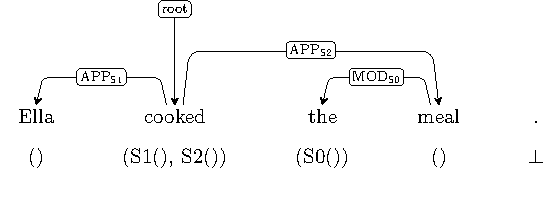
\includegraphics[scale=1.2]{figures/AM_dep_tree.pdf}
        \vspace{-1cm}
    \end{subfigure}

    \begin{subfigure}[t]{0.99\textwidth}
        \centering
        \vspace{-2cm}
        \raisebox{4\totalheight}{(b)}\phantomsubcaption\label{fig:b} 
        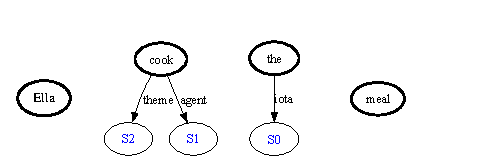
\includegraphics[scale=1.4]{figures/AM_supertags.pdf}
    \end{subfigure}
    \caption{Example of an AM dependency tree: (\subref{fig:b}) displays the supertags assigned to each token, while (\subref{fig:a}) presents the dependency tree connecting them.}
    \label{fig:supertag_example}
\end{figure}

To provide a valuable point of comparison, we finally evaluate a structure-informed model: AM-Parser \citep{groschwitz-etal-2018-amr}, which achieves near-perfect accuracy on COGS \citep{weissenhorn-etal-2022-compositional}. This allows us to measure how closely Transformer-based models can approximate the performance of a parser that explicitly incorporates compositional biases. Previous work has shown that structure-informed models perform well on compositional generalization tasks, specifically those involving structural generalization \citep{yao-koller-2022-structural}. Following \citet{weissenhorn-etal-2022-compositional}, we first have the AM-Parser predict an intermediate dependency tree (as shown in Figure~\ref{fig:supertag_example}), and then convert it to a graph-based representation of the SLOG logical form. The AM dependency tree labels each token with a \emph{supertag}, a small graph as illustrated in Figure~\ref{fig:b}, which captures the lexical meaning of each word. The tree's edges (Fig.~\ref{fig:a}) represent the compositional structure of the sentence, which specifies how the meaning of the sentence is recursively computed from the supertags.
For example, the second supertag in Figure~\ref{fig:b} represents the meaning of \textit{cooked} in the sentence \textit{Ella cooked the meal}. The blue markers ``S1'' and ``S2'' indicate that two arguments are needed to fill the agent and theme roles of \textit{cook}.

We use the A* AM-parser from \citet{lindemann-etal-2020-fast} for our experiments, as it yields the best overall results compared to alternative versions of AM-parser, such as the one in \citet{groschwitz-etal-2018-amr}.\footnote{For a more detailed discussion on alternative AM-parser models, please refer to Section~\ref{subsec:am_parser_analysis}.}

\vspace{-0.5\baselineskip}
\paragraph{Hyperparameters} 
The architecture of the vanilla Transformer model is the same as in original COGS, which consists of 2 encoder and 2 decoder layers, 4 attention heads per layer, and a feedforward dimension of 512. We use the best combination of hyperparameters from \citet{csordas-etal-2021-devil} on COGS: a learning rate of 0.0001 with no label smoothing, warmup, or early stopping. Absolute positional embeddings with down scaling scheme \citep{he2015delving,csordas-etal-2021-devil} is used due to stability issues observed with relative positional embeddings in recursive depth generalization cases, a similar phenomenon also noted in Csordas and colleague's experiments. Models are trained for 50k steps with a batch size of 128.

For the T5 experiments, we finetune T5-base\footnote{\url{https://huggingface.co/t5-base}} using a learning rate of 1.5e-5 and no label smoothing, warmup or early stopping. We finetune the model for 50k steps using a batch size of 2048.

For the LLaMA experiments, we finetune \texttt{llama-7b-hf} with LoRA \cite{hu2021lora}.\footnote{Low-Rank Adaptation of Large Language Models: \url{https://github.com/tloen/alpaca-lora}} We set the learning rate to 3e-4, LoRA rank to 8, alpha to 32 and dropout to 0.1. We finetune the model for 5K steps with a batch size of 64, with 100 warmup steps and no label smoothing or early stopping. We apply LoRA to ${W_q}$ and ${W_v}$ weight matrices in the model.

All our experiments were run five times, using different random seeds. The final checkpoints from each run were used for evaluation on both the in-domain test and out-of-domain generalization sets.

\subsection{Evaluation metric} 

Most studies report exact match accuracy on COGS. This metric has two limitations that may lead to an underestimation of a model's generalization capacity. First, because the COGS LF is conjunctive, any reordering of the conjuncts are semantically equivalent; yet, under exact match accuracy, only a single order is considered correct. Second, the COGS LF uses Skolem constants with a naming scheme tied to the linear indices of phrasal heads in the input. For example, in (\ref{ex:eval_ori_gold}), the constant saturating \lform{baby} is $x_3$ because, assuming 0-indexing, \textit{baby} appears in linear position 3 of the English expression \textit{What did the baby eat?}. While a commitment to a systematic naming scheme is necessary for consistent evaluation, different naming schemes up to the renaming of the constants in the gold LF yield equivalent LFs (e.g., (\ref{ex:eval_ori_gold}) vs. (\ref{ex:eval_ori_pred})). Such LFs would be considered incorrect under exact match.

To incorporate semantic equivalence up to conjunct reordering and constant renaming, at evaluation time, we alphabetically sort the conjuncts of the gold LFs, and subsequently index variables based on their appearance order in the sorted LFs. The same modifications are applied to the model output. This process results in the reformatted output as shown in (\ref{ex:eval_re}); applying these modifications to (\ref{ex:eval_ori_gold}) and (\ref{ex:eval_ori_pred}) yields the same outcome. Then, computing the exact match on these postprocessed LFs captures the targeted semantic equivalence.

\vspace{-0.5\baselineskip}
\begin{exe}
\ex \label{ex:eval_ori} Gold LF and model-predicted LF for \textit{What did the baby eat?}:
    \begin{xlist}
        \ex \label{ex:eval_ori_gold} Gold: \lform{eat.theme (x\textcolor{red}{$_4$}, ?) $\land$ eat.agent (x\textcolor{red}{$_4$}, x\textcolor{blue}{$_3$}) $\land$ baby (x\textcolor{blue}{$_3$})}
    \ex \label{ex:eval_ori_pred} Out: \lform{eat.agent (x\textcolor{red}{$_3$}, x\textcolor{blue}{\textcolor{blue}{$_6$}}) $\land$ eat.theme (x\textcolor{red}{$_3$},?) $\land$ baby(x\textcolor{blue}{\textcolor{blue}{$_6$}})}
    \end{xlist}
\ex \label{ex:eval_re} Re-indexed and re-ordered version: 
    \begin{xlist}
        \ex \lform{baby (y$_2$) $\land$ eat.agent (y$_1$, y$_2$) $\land$  eat.theme (y$_1$, ?)}  	
    \end{xlist}
\end{exe}
\vspace{-0.5\baselineskip}
\noindent This reformatted exact match metric is used for all results reported in the main text; see Appendix~\ref{app:metric} and Table~\ref{tab:res_cases} for more details. 

\section{Results} \label{sec:slog_res}

Overall, seq2seq Transformers, both trained from scratch and pretrained, display low accuracy on SLOG (Figure~\ref{fig:slog_cogs_res}), in line with earlier studies on structural generalization in seq2seq models \citep{yao-koller-2022-structural}. This is also the case for the more recent autoregressive Transformer LLaMa, whose performance is similar to that of T5. 



\begin{figure}[htbp]
  \centering
  \vspace{-4mm}  % reduce space above the figure
    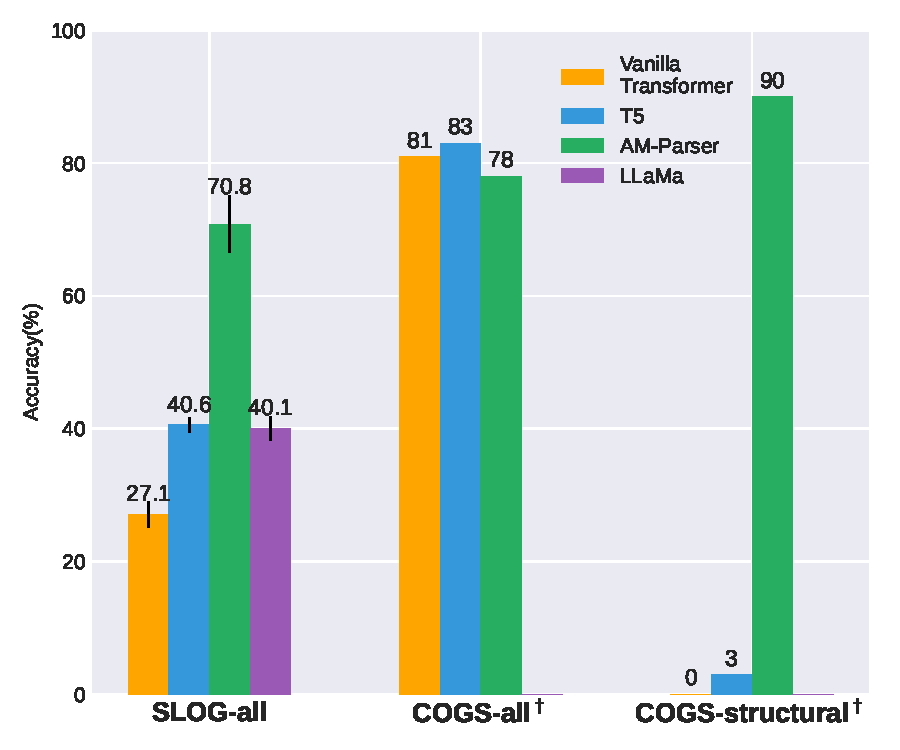
\includegraphics[scale=0.75]{figures/res_overall_slog_cogs.pdf}
    \vspace{-1mm} 
    \caption{Accuracy on SLOG, with error bars indicating variations across five runs. We also show the best published results on COGS (indicated with $^\dagger$), as reported in \citet{yao-koller-2022-structural}.}
    \label{fig:slog_cogs_res}
    \vspace{-2mm}  % reduce space below the figure
\end{figure}

\begin{figure}[H]
  \centering
  \vspace{-3mm} 
    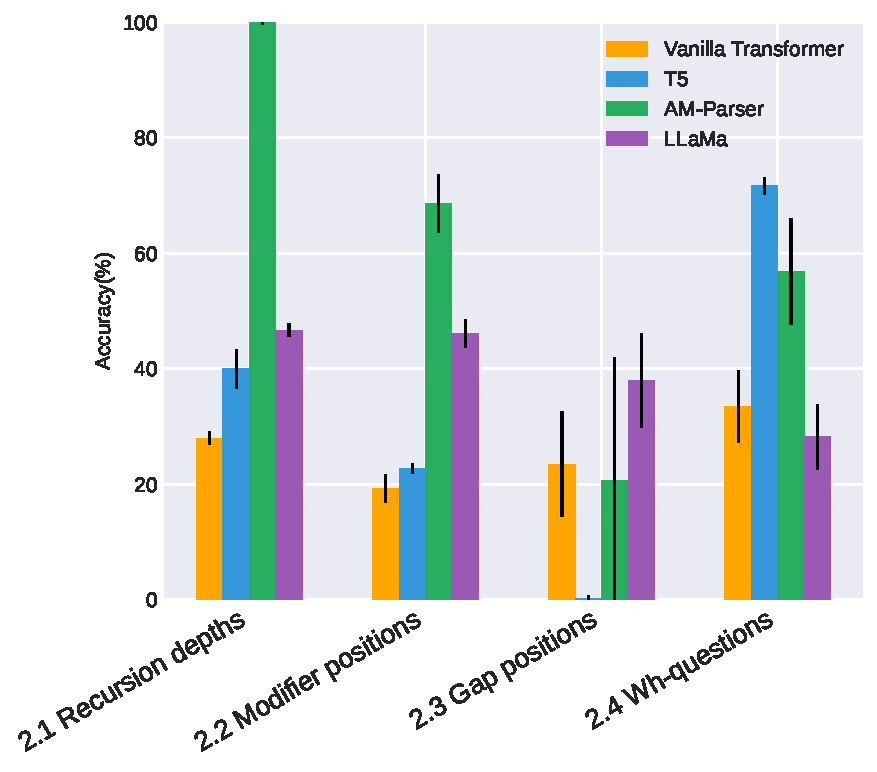
\includegraphics[scale=0.85]{figures/res_accuracy_category.pdf}
    \vspace{-1mm} 
    \caption{Aggregate accuracy on SLOG by generalization category, with error bars denoting the variations across generalization cases within each category over five model runs.}
    \label{fig:res_category}
    \vspace{-3mm} 
\end{figure}
 

As Figure~\ref{fig:slog_cogs_res} shows, high accuracy on the full COGS dataset, where 86\% of the generalization cases are lexical, can obscure low performance on structural generalization, highlighting the need for the expanded structural generalization tests included in SLOG.

SLOG additionally reveals weaknesses in the AM-Parser that COGS did not. While AM-Parser achieves 90\% accuracy on the structural generalization subset of COGS (Figure~\ref{fig:slog_cogs_res}), it faces systematic difficulties with several generalization types introduced in SLOG (Figure~\ref{fig:res_category}). We provide a detailed discussion of these difficulties in Section~\ref{subsec:am_parser_analysis}. 


Performance varied substantially across generalization categories (Figure~\ref{fig:res_category}); in particular, all models achieve near-perfect accuracy on \textit{Active subject wh-questions} and \textit{Shallower PP recursion}. These cases were the least structurally complex in their respective categories (\S\ref{subsec:cat_gap} and \S\ref{subsec:cat_recur}). 
We highlight several error patterns in individual generalization cases in more detail in the remainder of this section; see Appendix~\ref{sec:analysis_case} for full results and additional error analysis.


\subsection{Unobserved depth and length both affect depth generalization} \label{subsec:depth_gen}

The maximum depth observed in training was four levels of embedding for all three recursive structures tested. All models achieve greater than 90\% accuracy on unseen shallower PP recursion (three levels of embedding). A considerable lower performance is observed for Seq2Seq models with shallower tail CP recursion (<61\%); in particular, the vanilla Transformer consistently fails to generalize to shallower center embedding, with zero accuracy overall. Transformer models show systematically lower performance on deeper recursions (5-12 levels of embedding), whereas the structure-informed parsing model is robust to depth variation. 

\begin{table}[ht]
    \centering
    \begin{tabular}{lcccc}
    \toprule
     & \makecell[c]{Vanilla \\ Transformer} & T5 & LLaMa & \makecell[c]{AM \\parser} \\
    \midrule
     \textit{Within max training length}  &&&\\
    PP recursion & 29.3 &37.0 &46.0& 100.0 \\
    Tail CP recursion & 3.0 & 17.7&40.2& 100.0\\
    Center embedding & 0.0 & 0.0 &0.0& 100.0\\
    \midrule
    \textit{Beyond max training length }  &&&\\
    PP recursion & 0.0 &0.0 &0.0&100.0 \\
    Tail CP recursion & 0.0 & 0.0&0.0&100.0\\
    Center embedding & 0.0 &0.0&0.0&100.0 \\
    \bottomrule
    \end{tabular}
    \caption{Mean accuracy (\%) on unseen deeper recursion cases within and beyond the range of training output lengths (maximum training output = 229 tokens).}
    \label{tab:res_recursion}
\end{table}

We investigate the relation between length and depth generalization further by dividing the deeper depth generalization cases into examples that are shorter vs. longer than the maximum output length observed in training (229 output tokens). Results are shown in Table \ref{tab:res_recursion}. Both the vanilla Transformer and two pretrained  models are unable to generalize to examples longer than the maximum output length observed in training; this result is consistent with the difficulty of length extrapolation observed in the literature \citep{hupkes2020compositionality,anil2022exploring}. Length extrapolation does not capture the full story, however: their performance is limited even when the length of the generalization examples fall within the range of observed output lengths. This indicates that unobserved depth indeed plays a role in these models' poor generalization to deeper structures, in addition to known difficulties in length generalization.

\subsection{Unobserved long-distance dependencies make generalization difficult} \label{subsec:long_distance_hard}


Generalizing to subject modification (both PP and RC) is one of the most challenging cases in SLOG, Seq2seq models achieve near-zero accuracy, even with the additional cue from the standalone modified NPs that modification can appear outside of object positions. This challenge echoes previous findings on COGS \citep{akyurek-andreas-2021-lexicon,zheng-lapata-2022-disentangled,yao-koller-2022-structural}. The remainder of this subsection focuses on the analysis of PP modification cases, but similar patterns are observed for RC modifiers, which we discuss in Appendix \ref{app:RC_modifiers_results}.

Common error patterns across vanilla Transformer and two pre-trained models reveal a model bias towards shorter predicate-argument dependencies, which partly explains the difficulty of this generalization case. For instance, in sentences like \textit{A {\bf cat} on the mat {\bf froze}}, models often misinterpret the closer NP \textit{the mat} as the subject of \textit{froze}.

A further breakdown of the modifier generalization performance (Table~\ref{tab:cat_1_analysis}) illustrates the difficulty of long-distance dependencies clearly. As discussed in Section~\ref{subsec:cat_mod}, the sub-cases in indirect object modification feature predicate-argument dependencies of varying distance. We can see that generalization examples involving long predicate-argument dependency (i.e., there is an intervening non-argument NP between the predicate and the argument) tend to be more difficult for all models. However, the vanilla Transformer and pre-trained models show a stronger bias towards linearly adjacent predicate-argument structures.

\begin{table}[th]
    \centering
    \scalebox{0.85}{
    \begin{tabular}{lccccc}
      \toprule
       Generalization cases & \makecell[c]{Long pred-arg \\dependency?} & \makecell[c]{Vanilla \\Transformer} & T5 & LLaMa&\makecell[c]{AM \\parser}   \\
       \midrule
       \makecell[l]{ {\scriptsize Sub-case: Passive indirect objects} \\  \textbf{A fish} \textbf{was given} to  [ a cat on the mat ]$_{\textcolor{blue}{\bf iobj}}$. } & \ding{55}  & 95.5  & 97.5  & 98.2 & 93.6 \\
       \makecell[l]{ {\scriptsize Sub-case: Indirect object in PP datives  } \\   Emma \textbf{gave a fish} to  [ a cat on the mat ]$_{\textcolor{blue}{\bf iobj}}$.} & \ding{55} & 22.9  & 50.5 & 75.5 & 100.0  \\
      \makecell[l]{ {\scriptsize Sub-case: Indirect object in double object datives} \\    Emma \textbf{\textcolor{orange}{gave}} [ a cat on the mat ]$_{\textcolor{blue}{\bf iobj}}$ \textbf{\textcolor{orange}{a fish}}.} & \ding{51} & 4.5 & 9.7  &36.3 & 77.9 \\
      \makecell[l]{ {\scriptsize Subject} \\ \  [\textbf{\textcolor{orange}{A cat}} on a mat]$_{\textcolor{blue}{\bf subj}}$ \textbf{\textcolor{orange}{ate}} a fish. } & \ding{51} & 0.0 & 0.8 &28.9&57.6\\
      \bottomrule
    \end{tabular}    
    }
    \caption{Performance of PP modification generalization broken down by construction. Bold orange words denote long predicate-argument dependencies, while bold black words indicate short ones.} 
    \label{tab:cat_1_analysis}
\end{table}

For both constructions involving long predicate-argument dependencies, indirect object position seems less challenging than subject position. A possible explanation is that the former has a closer surface resemblance to direct object modification~---~modifiers attach to an immediate post-verb NP. Indeed, we observe that a higher proportion of indirect object modifications are partially correct; models correctly predicted the PP-modified NP, but erred in the argument structure. 

We furthermore note that the results in Table~\ref{tab:cat_1_analysis} also show lower performance of Transformer models for \textit{Indirect object in PP datives} compared to \textit{Passive indirect objects}, although neither subcase introduces long predicate-argument dependencies. The predominant error pattern in the former subcase is the incorrect attachment of PP modifiers to the direct object NP. For example in (\ref{ex:iobj_a_dobj_pred}), NP inside the modifier \textit{on the mat} denoted by \lform{$x_9$} was attached to \textit{a fish} instead of \textit{the cat}. This suggests that Transformers additionally apply the incorrect modification rule ``attach PPs to NPs in immediate post-verb position'', which is compatible with the training data but does not lead to correct generalization. 

\begin{exe}
\ex \label{ex:iobj_error} Gold LF and model-predicted LF for \textit{Emma gave a fish to the cat on the mat}:
    \begin{xlist}
        \small{
        \ex \label{ex:iobj_a_dobj_gold} Gold: \lform{*cat ($x_6$); *mat($x_9$); \\ give.agent ($x_1$,Emma) $\land$ give.theme ($x_4,x_3)$ $\land$  give.recipient ($x_1,x_6$)$\land$ fish($x_3$) $\land$ \textbf{cat}.nmod.on (x\textcolor{red}{$_6$}$,x_9$)}
    \ex \label{ex:iobj_a_dobj_pred} Out: \lform{*cat ($x_6$); *mat($x_9$); \\ give.agent ($x_1$,Emma) $\land$ give.theme ($x_4,x_3)$ $\land$  give.recipient ($x_1,x_6$)$ \land$ fish($x_3$) $\land$ \textbf{fish}.nmod.on (x$\textcolor{red}{_3},x_9$)}
    }
    \end{xlist}
\end{exe}


\subsection{Gap generalizations are challenging for all tested models} \label{subsec:am_parser_analysis}

All tested models encounter significant difficulties with gap constructions, as evidenced by their low accuracy and considerable variability across runs. In the case of indirect object-extracted relative clauses (\ref{ex:RC_iobj_extracted}), a common error pattern emerges across all models: they tend to mirror the training pattern of direct object-extracted RCs, as demonstrated by the incorrect output (\ref{ex:RC_iobj_extracted_error}). In contrast, when handling \emph{wh}-questions, the models show distinct difficulties, revealing varied error patterns.

\begin{exe}
    \ex \label{ex:RC_iobj_extracted} Input: Ella cooked the servant that Emma gave a tool to \_\_.
    \begin{xlist}
    \ex \label{ex:RC_iobj_extracted_gold} Gold: \lform{*servant($x_3$);cook.agent($x_1$, Ella) $\land$ cook.theme($x_1, x_3$) \\ $\land$  servant.nmod( $x_3, x_6$) $\land$ give.agent($x_6$, Emma) $\land$ give.theme ($x_6,\textcolor{blue}{x_8}$) \\ $\land$ 
    give.recipient($x_6,x_3$) $\land$ tool ($\textcolor{blue}{x_8}$)}
    \ex \label{ex:RC_iobj_extracted_error} Models output: \lform{*servant($\textcolor{red}{x_3}$);cook.agent($x_1$, Ella) $\land$ cook.theme($x_1, x_3$) $\land$ servant.nmod( $x_3, x_6$) $\land$ give.agent($x_6$, Emma) $\land$ give.theme ($x_6,\textcolor{red}{x_3}$) $\land$ give.recipient($x_6,x_8$) $\land$ tool ($x_8$)} 
    \end{xlist}
\end{exe}

\paragraph{Direct and indirect \textit{wh}-questions}The vanilla Transformer and LLaMa frequently misinterpret the theme role in direct object \emph{wh}-questions. For example, they often fail to map \emph{wh}-words to `?' as illustrated in (\ref{ex:q_error_tm}):  
\begin{exe}

\ex \label{ex:q_input}Input: What did Emma sell to Liam ?
%\vspace{-0.4em}
\small{\begin{xlist}
    \ex \label{ex:q_gold} Gold:\lform{sell.theme (x$_3$, ?)$\land$ sell.agent (x$_3$, Emma) $\land$ sell.recipient(x$_3$,Liam)}
    \ex \label{ex:q_error_tm} Output of vanilla Transformer and LLaMa: \\ \lform{sell.theme (x$_3$,  \textcolor{red}{x$_3$}) $\land$ sell.agent (x$_3$, Emma)$\land$ sell.recipient(x$_3$,Liam)}
    \ex \label{ex:q_error_am} AM parser's output: \\ \lform{sell.\textcolor{red}{agent} (x$_3$,  ?) $\land$ sell.\textcolor{red}{theme} (x$_3$, Emma)$\land$ sell.recipient(x$_3$,Liam)}
\end{xlist}}
\end{exe}

\noindent This error pattern can be traced back to frequency of the subsequences in the training data. Three types of tokens can appear post-comma in the output LF space: \lform{$x$}, \lform{?} (denoting \emph{wh}-words), or a proper noun (\lform{PropN}), such as \lform{Emma}. The subsequence \texttt{theme($x_i,x_j$)} is 20 times more frequent than \texttt{theme($x_i$,?)} and \texttt{theme($x_i$,PropN)}. This discrepancy does not affect all models equally; in fact, T5 can generalize correctly for some constructions despite this skewed label distribution, achieving near-perfect accuracy for direct object \emph{wh}-questions. However, when it comes to less frequent constructions --- indirect object \emph{wh}-questions, T5 overgeneralizes. In 94.6\% of these cases, it erroneously produces the observed direct object \emph{wh}-questions pattern \texttt{theme(x$_i$,?)}, instead of the correct but unseen \texttt{recipient(x$_i$,?)}. This observation aligns with the findings of \citet{wu2023recogs,yao-koller-2022-structural}, who noted that the decoder of Transformer models tends to exhibit a heavy bias towards generating observed $n$-grams.

\begin{figure}[ht] 
    \centering

    \begin{subfigure}[t]{0.99\textwidth}
        \centering
        \raisebox{4\totalheight}{\phantom{(abc)}}\phantomsubcaption
        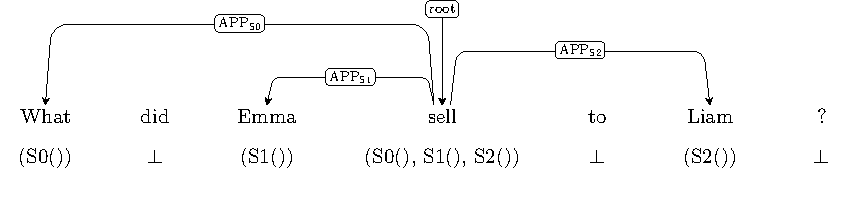
\includegraphics[scale=0.97]{figures/dobj_Q_deptree.pdf}
        \vspace{-1cm}
    \end{subfigure}
    \setcounter{subfigure}{0}  % Reset the subfigure counter
    \begin{subfigure}[t]{0.99\textwidth}
        \centering
        \vspace{-1.5cm}
        \raisebox{3\totalheight}{(a)}\phantomsubcaption\label{fig:dobj_Q_gold} 
        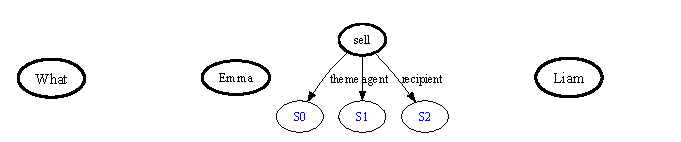
\includegraphics[scale=1.2]{figures/dobj_Q_gold_supertags.pdf}
    \end{subfigure}
    \begin{subfigure}[t]{0.99\textwidth}
        \centering
        \vspace{-0.5cm}
        \raisebox{3\totalheight}{(b)}\phantomsubcaption\label{fig:dobj_Q_error} 
        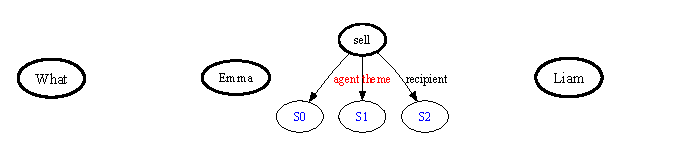
\includegraphics[scale=1.2]{figures/dobj_Q_error_supertags.pdf}
    \end{subfigure}
    \caption{AM dependency tree for a direct object \textit{wh}-question. (\subref{fig:dobj_Q_gold})  displays the gold supertags and (\subref{fig:dobj_Q_error}) shows the incorrect predicted supertags. }
    \label{fig:dobj_deptree}
\end{figure}


AM-Parser shows considerable fluctuation in performance across different runs on the indirect and direct object \textit{wh}-questions cases, with accuracies ranging from 0 to 80 depending on the random seed. This is because at the bottom of its compositional process, the AM-Parser predicts the lexical meaning for each token in the sentence (\textit{supertag}). In these generalization types, the gold meaning representations in the test set require supertags that are infrequent in training. 

We show an example of AM dependency trees for an \textit{direct object wh-question} sentence in Figure \ref{fig:dobj_deptree}, with gold supertags in Figure~\ref{fig:dobj_Q_gold} and predicated supertags in Figure~\ref{fig:dobj_Q_error}. The issue here is that the model predicts the wrong supertag for \emph{sell}, treating \emph{What} as its \texttt{agent} instead of \texttt{theme}, and \emph{Emma} as its \texttt{theme} rather than \texttt{agent}, which results in the erroneous output LF as shown in (\ref{ex:q_error_am}). The AM-Parser is limited to using supertags that it observed at training time (possibly with different node labels to accommodate novel lexical material). In this case, the correct supertag was actually present in the training data, but it was much less frequent than the one in Figure~\ref{fig:dobj_Q_error}. We conjecture that the AM-Parser was overly sensitive to the supertag distribution in the training data in this case, pointing to a further architectural limitation. 

Thus, while the AM-Parser can compensate the distribution shift of the meaning representations as a whole, SLOG exposes its weakness to distribution shifts in the lexical supertags. 





\paragraph{\textit{Wh}-questions with long movement} 
All models achieve very low accuracy when generalizing to longer filler-gap dependency across CPs.

In example (\ref{ex:q_long_mv_tm}), we show an example of a \textit{wh-question with long movement}, with its gold meaning representation (\ref{ex:q_long_mv_gold}) and the most common errors produced by Transformer-based models. As shown in (\ref{ex:q_long_mv_tm}), the vanilla Transformer commonly misinterprets the complementizer \textit{that} (corresponding to \texttt{ccomp} in the LF) as a relative pronoun (\texttt{nmod}). Additionally, it tends to interpret the \emph{wh}-word as the direct object of the CP verb, \emph{e.g., say}. In the most common errors for T5 and LLaMa (\ref{ex:q_long_mv_t5}), the whole gap conjunct (\lform{paint.theme($x_7,?$)}) is missing, revealing their difficulties in establishing long-range filler-gap dependencies between the initial \emph{wh}-word and the embedded gap position. 
 
\begin{exe}
\ex \label{ex:q_long_mv_input}Input: What did Liam say that the bear painted \_\_ ?
\begin{xlist}
    \ex \label{ex:q_long_mv_gold} Gold:  \lform{*bear(x$_6$); say.agent(x$_3$,Liam) $\land$ say.ccomp(x$_3$,x$_7$) $\land$ \\ paint.agent(x$_7$,x$_6$) $\land$ paint.theme(x$_7$,?)}
    \ex  \label{ex:q_long_mv_tm} Output of vanilla Transformer:  \lform{*bear(x$_6$); say.agent(x$_3$,Liam) $\land$ \\ \textcolor{red}{say.theme(x$_3$,?)} $\land$ say.\textcolor{red}{nmod}(x$_3$,x$_7$) $\land$ paint.agent(x$_7$,x$_6$) $\land$ \\ paint.theme(x$_7$,?)}
    \ex \label{ex:q_long_mv_t5} Output of T5 and LLaMa:  \lform{*bear(x$_5$); say.agent(x$_3$,Liam) $\land$ \\ say.ccomp(x$_3$,x$_7$) $\land$ paint.agent(x$_7$,x$_5$) }
\end{xlist}
\end{exe}

The AM parser fails on all test instances in the case of \textit{wh-questions with long movement}. We present a predicted AM dependency tree for such a sentence in Figure \ref{fig:predicted_Q_long_mv}, contrasted with the corresponding gold standard AM dependency tree in Figure \ref{fig:gold_Q_long_mv}. Notably, for \textit{wh}-questions with long movement, the required dependency trees are nonprojective, as illustrated in Figure \ref{fig:gold_Q_long_mv}: the edge from the embedded verb to the \textit{wh}-pronoun (the edge \texttt{snapped -> Who}) crosses the matrix verb (\texttt{root -> appreciate}). However, the A* AM-Parser used in our study only supports projective dependency trees, leading to incorrect prediction of sentence structure as shown in Figure \ref{fig:predicted_Q_long_mv}.\footnote{Instead of the A* parser, one could instead use the fixed-tree decoder of \citet{groschwitz-etal-2018-amr}, which is capable of predicting non-projective
AM dependency trees. This parser achieves nonzero accuracy (36\%) on \textit{wh}-questions with long movement,
confirming our hypothesis that the projectivity is the issue. However, the A* parser
outperforms the fixed-tree decoder on most other generalization types, which is why
we only report its results in the main body of the paper. The transition-based
AM-Parser of \citet{lindemann-etal-2020-fast} can also predict non-projective trees,
but uses a different probability model that is incompatible with the training algorithm
of \citet{groschwitz-etal-2021-learning} that we use here.}

\begin{figure}[ht]
    \centering
    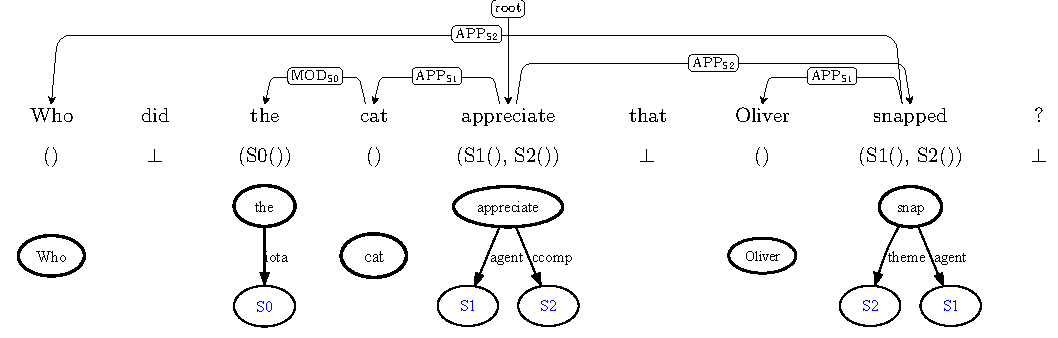
\includegraphics[scale=0.85]{figures/am_deptree_Q_long_mv.pdf}
    \caption{Example of gold AM dependency tree for \textit{wh}-questions with long movement}
    \label{fig:gold_Q_long_mv}
\end{figure} 

\begin{figure}[ht]
    \centering
    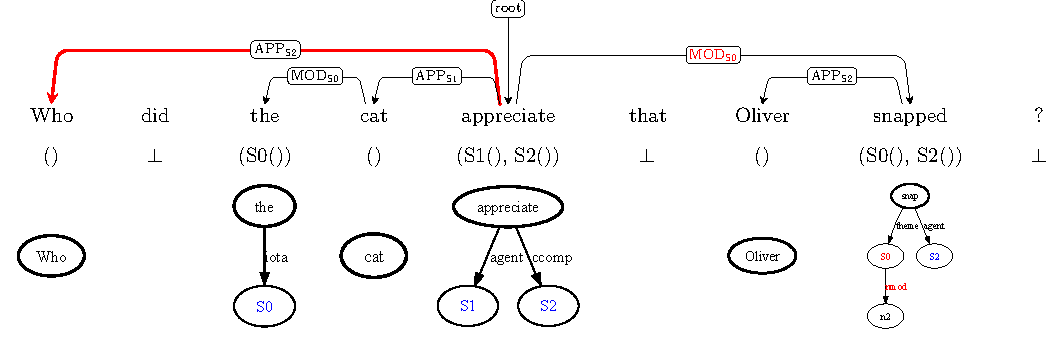
\includegraphics[scale=0.85]{figures/am_deptree_Q_long_mv_error.pdf}
    \caption{Example of predicted AM dependency tree for \textit{wh}-questions with long movement}
    \label{fig:predicted_Q_long_mv}
\end{figure} 


Note that the A* AM-Parser's limitation to projective structures is shared by many other compositional semantic parsers. For instance, the LeAR model of \citet{liu-etal-2021-learning-algebraic} uses phrase-structure trees as compositional structures. Similarly, the CSL-T5 parser of 
\citet{qiu-etal-2022-improving} uses phrase-structure trees during the data augmentation process. Since phrase structure trees are equivalent to projective dependency trees, these parsers are likely to encounter similar difficulties on SLOG.
Thus, this specific type of generalization can serve as a diagnostic tool to identify structural limitations in compositional semantic parsers.

\clearpage
\section{Conclusion} \label{sec:slog_conclu} 

Transformer-based models, despite lacking explicit symbolic representation, have demonstrated a remarkable ability to acquire nuanced syntactic representations, enabling them to handle structure-sensitive phenomena effectively, as discussed in Chapter~\ref{chp:main_project}. To further probe the extent to which their performance is driven by genuine syntactic generalization, aligned with symbolic compositional rules, as opposed to relying on structural similarity-based memorization derived from their training data, we introduced SLOG. This semantic parsing challenge set expands upon the COGS benchmark, and specifically targets structural generalization, which is often underrepresented in current compositional generalization benchmarks. 

Using SLOG, we assessed the structural generalization capacity of Transformer models (both pretrained and trained from scratch), as well as AM-Parser, a structure-informed parsing model. While all models achieve good overall accuracy on COGS ($\geq$ 78\%), their performance on SLOG is substantially lower. This was particularly evident for Transformer models, which scored below 41\%, lagging behind the structure-informed parser (70.8\%) by a wide margin. This performance discrepancy between SLOG and COGS illuminates the notable gap between models' lexical and structural generalization abilities. 

Prior studies have shown that RNN models often struggle with learning complex long-range relations from simpler formal languages \citep{avcu2017subregular, mahalunkar-kelleher-2019-multi}. Our results on SLOG reveal that unseen long-distance predicate-argument dependencies pose considerable difficulty for Transformer-based models as well (\S\ref{subsec:long_distance_hard}). 
Additionally, these Transformer models struggle with deeper recursive constructions. Our results corroborate the observations of \cite{hupkes2020compositionality} and \cite{lakretz2021can}, and further highlight challenges posed by unobserved deeper patterns, which persist beyond the recognized issue of length extrapolation~(\S\ref{subsec:depth_gen}). On the other hand, the AM-Parser, despite its stronger overall performance (70.8\%), displays categorical failures on gap generalization due to its inherent parser design limitations (\S\ref{subsec:am_parser_analysis}). 

These findings underscore the utility of SLOG in exposing the limitations of current semantic parsing models, which have previously been claimed to achieve good compositional generalization. SLOG thus can serve as a useful analytic tool for guiding future improvements. Furthermore, these results indicate that while Transformer-based models can approximate compositional behavior to a certain extent, they do not seem to rely on the kind of syntactic generalization rooted in systematic compositional rules. This insight lends support to the hypothesis that the Transformer model's ability to leverage hierarchical structures for nuanced syntactic generalization, as explored in Chapter~\ref{chp:main_project}, might be more attributable to structural similarity-based analogies at the lexico-categorical abstraction level, rather than the internalization and application of systematic grammatical rules. This enables the models to handle a sophisticated form of language productivity; however, they falter when faced with novel linguistic structures that require the induction of systematic compositional rules.

The evaluation conducted with the SLOG challenge set represents only the first step --- behavioral level --- of our integrated three-level analysis framework as detailed in Chapter~\ref{chp:main_project}. This study thereby lays the groundwork for future research, particularly aimed at understanding what makes structural generalization so hard for Transformer models. The logical progression would be to advance to the representational and functional levels of analysis, using probing classifiers and causal intervention methodologies to delve into the model's difficulties with SLOG. 

\stopcontents[chapters]